\begin{figure}
  \centering
  \begin{tabular}{ccc}
    \begin{minipage}{0.330\hsize}
      \centering
      $\pi^-\Sigma^+$ mode
      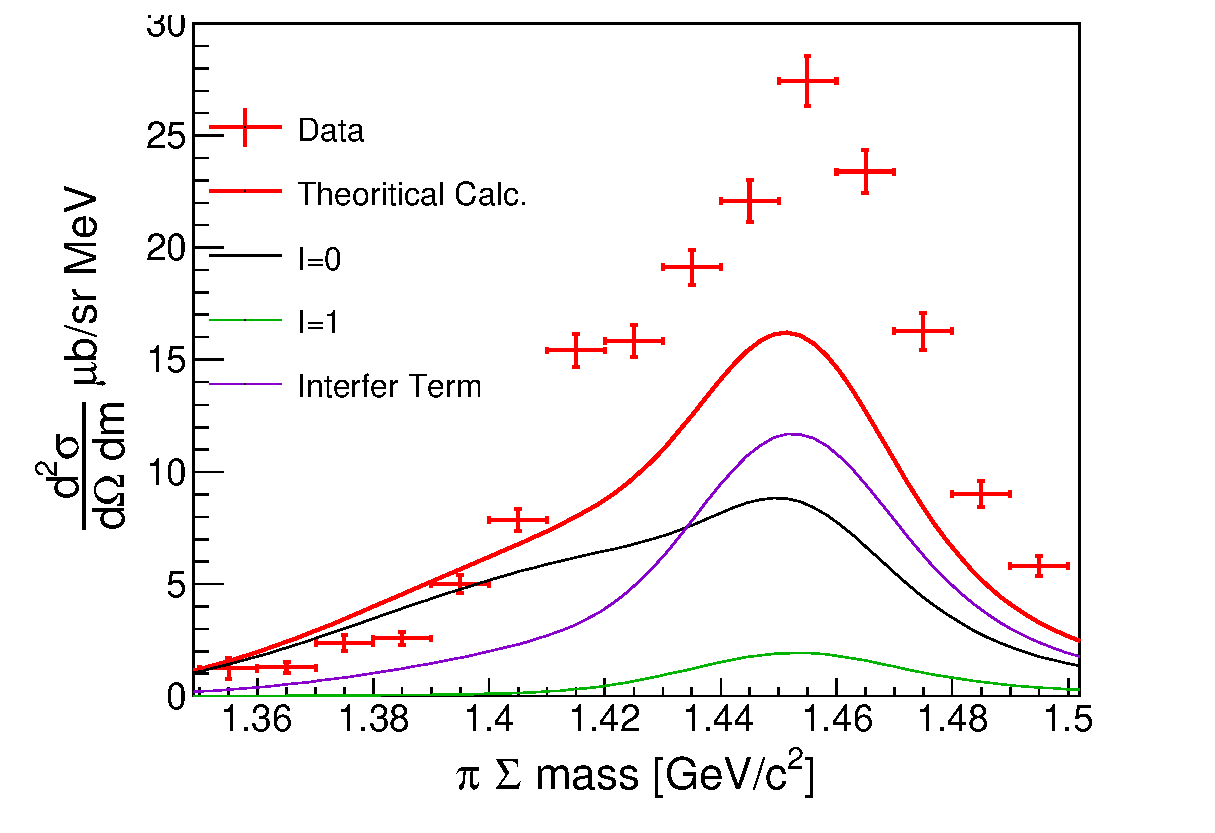
\includegraphics[width=4.5cm]{../pic/Dron/fit_model_B_2/pimSp_fit.eps}
    \end{minipage}

    \begin{minipage}{0.33\hsize}
      \centering
      $\pi^+\Sigma^-$ mode
      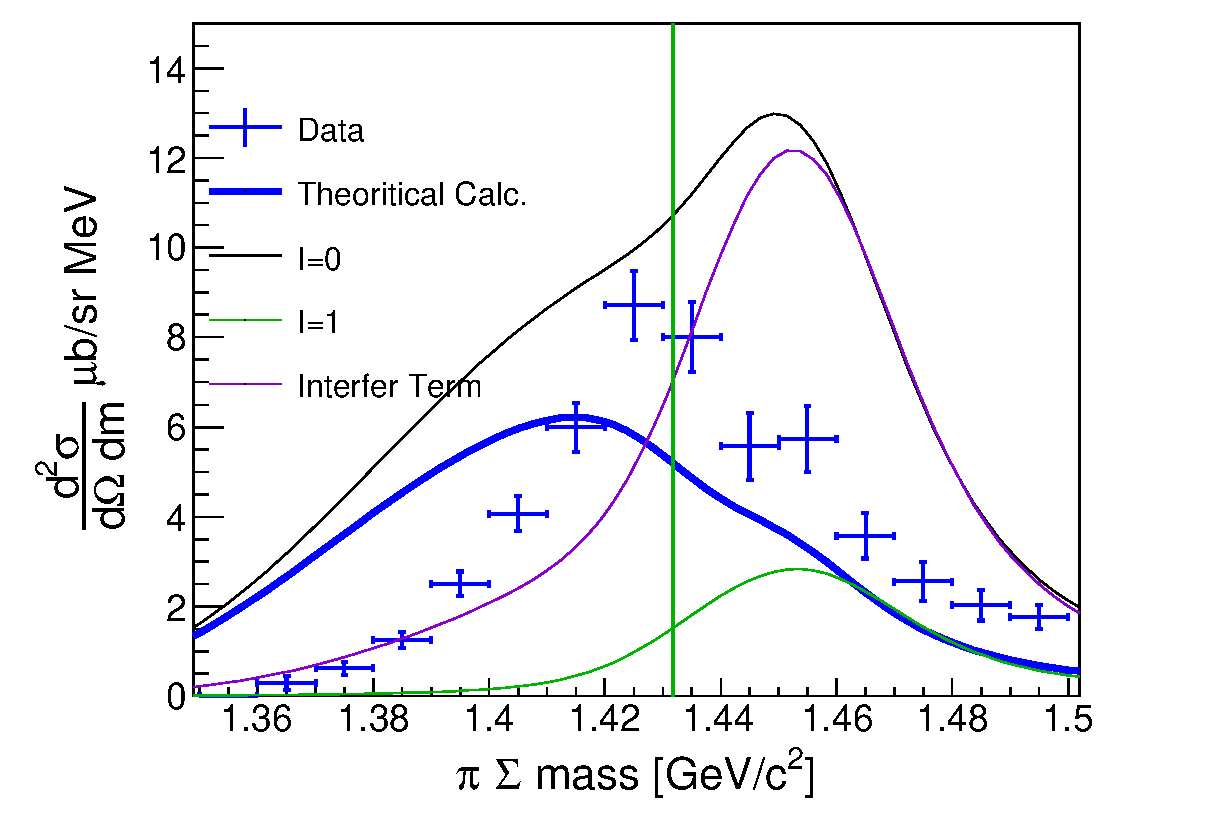
\includegraphics[width=4.5cm]{../pic/Dron/fit_model_B_2/pipSm_fit.eps}
    \end{minipage}

    \begin{minipage}{0.33\hsize}
      \centering
      $\pi^-\Sigma^0$ mode
      \includegraphics[width=4.5cm]{../pic/Dron/fit_model_B_2/pimS0_fit.eps}
    \end{minipage}
  \end{tabular}

  \begin{tabular}{cc}
    \begin{minipage}{0.5\hsize}
      \centering
      $I=0$\\
      \includegraphics[width=4.5cm]{../pic/Dron/fit_model_B_2/I0_fit.eps}
    \end{minipage}
    
    \begin{minipage}{0.5\hsize}
      \centering
      Interfer\\
      \includegraphics[width=4.5cm]{../pic/Dron/fit_model_B_2/interfer_fit.eps}
    \end{minipage}
  \end{tabular}
  \caption{
    These figures shows result of the fitting, in which $I=1$ is decided by $\pi^-\Sigma^0$ and $I=0$ and interference term are determined after.
    The figure notation is same as Fig.[\ref{fig:fit_A_scale}].
  }
  \label{fig:fit_B_fix_phase}
\end{figure}
